%_____________________________________________________________________________________________ 
% LATEX Template: Department of Comp/IT BTech Project Reports
% Sample Chapter
% Sun Mar 27 10:25:35 IST 2011
%
% Note: Itemization, enumeration and other things not shown. A sample figure is included.
%_____________________________________________________________________________________________ 

\chapter{Introduction}
\section{What is a Chatbot?}
A chatbot is a “human-computer dialog system with natural language.”  A basic
framework that outlines the functions expected from modern chatbots can be
described as:

\begin{itemize}[align=left]
	\item [\textbf{A. Dialogic Agent:}] It must understand the user, i.e. it
		must provide the function of comprehension. Bots are provided
		with a textual input, which should be analyzed and generate
		appropriate responses.

	\item [\textbf{B. Rational Agent:}] It must have access to an external
		base of knowledge and common sense i.e huge datasets such that
		it can provide the function of competence and answering user
		questions. It should store context-specific information
		including but not limited to the user’s personal details, some
		event the user is currently referring to, etc.

	\item [\textbf{C. Embodied Agent:}] It should “provide the function of
		presence”. This was earlier considered to be optional, but today
		it is considered to be critical for the product to be accepted
		by the users at large. Today, developers are focused on the use
		of language tricks to create personas for chatbots in order to
		build trust with users and give the impression of an embodied
		agent.

\end{itemize}

%Th is is a section. We can cite a reference like this: \cite{INTERNET} 	
						% Citation. See references.tex for the entry.
\section{History of Chatbots}
In 1950, Alan Turing asked the question “Can machines think?”. Turing
conceptualized the problem as an ‘imitation game’ (Turing Test), in which an
‘interrogator’ asked questions to human and machine subjects, with the goal of
identifying the human. If the human and machine are indistinguishable, he said
that we could conclude that the machine could think. 

In 1966, Joseph Weizenbaum at MIT created the first chatbot that, arguably, came
close to imitating a human: ELIZA. Given an input sentence, ELIZA would identify
keywords and pattern match those keywords against a set of pre-programmed rules
to generate appropriate responses. 

Since ELIZA, there has been progress in the development of increasingly
intelligent chatbots. In 1972, Kenneth Colby at Stanford created PARRY, a bot
that impersonated a paranoid schizophrenic. In 1995, Richard Wallace created
A.L.I.C.E, a significantly more complex bot that generated responses by pattern
matching inputs against <pattern> (input) <template> (output) pairs stored in
documents in a knowledge base. These documents were written in Artificial
Intelligence Markup Language (AIML), an extension of XML, which is still in use
today. 

Modern chatbots include: Amazon’s Echo and Alexa, Apple’s Siri, and Microsoft’s
Cortana. The architectures and retrieval processes of these bots take advantage
of advances in machine learning to provide advanced “information retrieval”
processes, in which responses are generated based on analysis of the results of
web searches. Others have adopted “generative” models to respond; they use
Statistical Machine Translation (SMT) techniques to “translate” input phrases
into output responses. Seq2Seq, an SMT algorithm that used recurrent neural
networks (RNNs) to encode and decode inputs into responses is a current best
practice.

\section{Question Answering Chatbot}
A Question Answering Chatbot is a kind of chatbot specifically designed only to
answer questions posed by the user. The major difference between usual chatbots
and a QA chatbot is that the QA chatbot is specifically designed only to answer
user’s questions and not for its other purposes like carrying out commands or
performing repetitive tasks. It can be used to answer general questions like
those from current events, news articles or those from specific domains only
like astrology, astronomy, etc. 


\subsection{Types of QA Chatbot}
QA research attempts to deal with a wide range of question types including:
fact, list, definition, How, Why, hypothetical, semantically constrained, and
cross-lingual questions. There are two type of questioning answering system:

\subsection*{Closed Domain:}
Closed Domain system deals with questions under a specific domain like biology
or cricket. Closed-domain might refer to a situation where only limited types of
questions are accepted. NLP systems that can exploit domain-specific knowledge
frequently formalized in ontologies make this task easier. 

\subsection*{Open Domain:}
Open Domain systems rely on word knowledge and general ontologies and deals with
questions about nearly any topic of human interest. Plenty of datasets can be
found available for training purposes of such chatbots.

\section{Architecture \& Design}
\subsection{Natural Language Processing}
The goal of natural language processing (NLP) is to take the unstructured output
and produce a structured representation of the text that contains natural
language understanding (NLU). In this section, we explore a number of methods
for extracting semantic information from written language in order to create
grammatical data structures that can be processed by the Dialogue Management
unit in the next step.  Likewise, text inputs to a chatbot may contain (i)
grammatical mistakes, (ii) disfluencies, (iii) interruptions, and (iv)
self-corrections.

\paragraph{Dialogue Act (DA) Recognition}

One way to extract meaning from natural language is to determine the type of the
sentence. The common classification can be made as Assertive, Interrogative,
Imperative, Conventional Opening or Exclamatory. Such a classification of
sentences is referred to as Dialogue Act Recognition. 

In dialogue act recognition systems, a corpus of sentences (training data) is
labeled with the function of the sentence, and a statistical machine learning
model is built which takes in a sentence and outputs its function. The model
uses a number of different features to classify the sentences including but not
limited to words and phrases such as ‘please’ or ‘are you’ syntactic information
like position of subject and object of verb, etc.

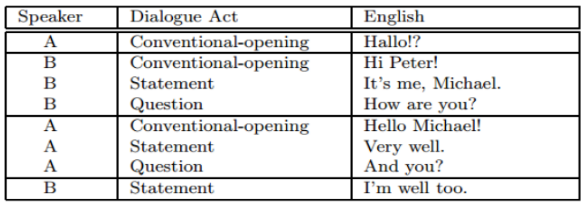
\includegraphics[width=\linewidth]{1.png}


\paragraph{Bayesian Approaches to DA Models}

The idea behind using a Bayesian approach to DA models is to find the
probability of every possible sequence of dialogue acts DA that could represent
a sentence, and find the dialogue act sequence with the highest probability of
occurring.

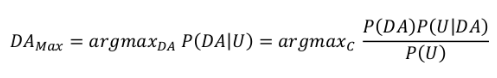
\includegraphics[width=\linewidth]{2.png}
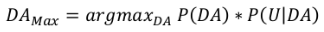
\includegraphics[width=\linewidth]{3.png}

Assuming the N individual words of the sentence are known, using the Naïve Bayes
assumptions of independence of subsequent words holds, this leads to:

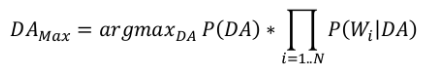
\includegraphics[width=\linewidth]{4.png}

This is the unigram model, where P(DA) and P(Wi |DA) can be quantified from
empirical data. Using this Naïve Bayes classifier, 74\% accuracy rate for
classifying the correct dialogue act from a given sentence can be obtained.
N-gram models are frequently used to include dialogue history in the model.
These models estimate P (DA | N historical DAs) rather than P(DA). 

Hidden Markov Models can also be used to model dialogue history, where each
state represents a dialogue act in the conversation history of the chatbot.
Likewise, neural network classifiers can be trained as well. A combination of
HMMs and neural networks has achieved 76\% accuracy.

\paragraph{Information Extraction}

The primary responsibility of the NLU is to understand the meaning of the text
itself and not just individual phrases. To extract meaning from text, we convert
unstructured text  into structured grammatical data objects, which will be
further processed by the Dialogue Manager. The first step in this process is
breaking down a sentence into tokens that represent each of its component parts:
words, punctuation marks, numbers, etc. Tokenization is difficult because of the
frequency of ambiguous or malformed inputs including: (i) phrases (e.g. New
York), (ii) contractions (e.g. aren’t), abbreviations (e.g. Dr.), and periods
(e.g. distinguishing those used in “Mr.” and at the end of a sentence). These
tokens can be analyzed using a number of techniques, described below, to create
a number of different data structures that be processed by the dialogue manager.

\paragraph*{Bag of Words:}

Here the sentence structure, order, and syntax is ignored and only the number of
occurrences of each word. Stop words are removed from the corpus and
lemmatization is carried out. The final bag of words are reduced to a vector
space, with each distinct word representing an axes. In the dialogue manager
phase, assuming a rule-based bot, these resulting words will be matched against
vectors stored in the bot’s knowledge database to find those with inputs
containing similar keywords. The bag of words approach is simple but is not
precise enough to solve complex problems.

\paragraph*{Latent Semantic Analysis (LSA):}

This approach is similar to the bag of words. Meanings instead of words, are the
basic unit of comparison parsed from a given sentence. Second, groups of words
that co-occur frequently are grouped together. In LSA, we create a matrix where
each row represents a unique word, each column represents a document, and the
value of each cell is the frequency of the word in the document. The distance
between the vector representing each utterance and document, using singular
value decomposition (reducing the dimensionality of the matrix) is computed and
the closest document is determined. 

\paragraph*{Regular Expressions:}

Sentences can be treated as regular expressions, and can be pattern matched
against the documents in the bot’s knowledge database. For example, imagine that
one of the documents in the bot’s knowledge database handles the case where the
user inputs the phrase: ‘My name is \_.’ where “\_” is the wildcard character,
indicates that this regular expression should be triggered whenever the bot
hears the phrase “my name is” followed by any word. 

\paragraph*{Part of Speech (POS) Tagging:}

POS tagging labels each word in the input string with its part of speech. These
labels can be rule-based or can also be created using stochastic models which
train on sentences labeled with correct POS. POS tagging has plenty of uses in
information extraction. In the dialogue manager, POS can be used to store
relevant information in the dialogue history. POS is can be used in response
generation to indicate the POS object type of the desired response.

%img
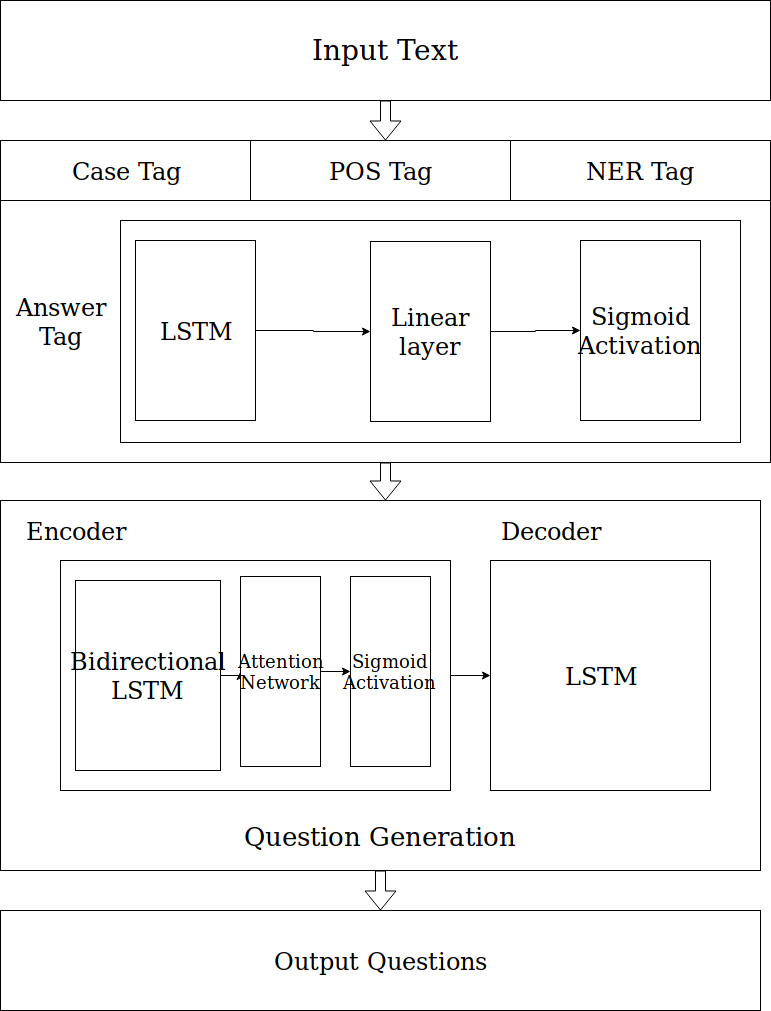
\includegraphics[width=\linewidth]{5.png}

Named Entity Recognition(NER): In Named Entity Recognition, the names of people,
places, groups, and locations are extracted and labeled accordingly. NER-name
pairs can be stored by the dialogue manager in the context history to keep track
of the context of the bot’s current context. Relation extraction goes one step
further to identity relations like “Who did what to whom” and label each word in
these phrases accordingly.

%img
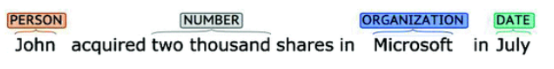
\includegraphics[width=\linewidth]{6.png}

Creation of Grammatical Data Structures: Sentences and utterances can be stored
in a structured way in grammar formalisms such as context-free grammars (CFGs).
Context-free grammars are tree-like data structures that represent sentences as
containing noun phrases and verb phrases, each of which contain nouns, verbs,
subjects, and other grammatical constructs. Dependency grammars, by contrast,
focus on the relationships between words.

\subsection{Methodology}
\paragraph{AIML Chat Bot Implementation}
AIML chat bot, also known as alice bot is a very simple to use chat bot which
could be customized to operate for answering simple FAQ type of questions. It
could be changed to reverse the process ,i.e. to create questions given a topic.
For this all the documents containing the information about a particular topic
is processed to acquire all the sentences on which questions can be generated.
The statement can be used to generate questions based on some patterns. It has
the following basic tags.

\begin{itemize}[align=left]
	\item [<aiml>]: This tag begins and ends the AIML chatbot document

	\item [<Category>]: This tag marks a "unit of knowledge" in the bot’s knowledge base.

	\item [<Pattern>]: This tag is used to contain a simple pattern that matches user input
given to an Alicebot. These pattern tags store the context of the conversation
and are really useful for a successful chat bot implementation.

	\item [<Template>]: This tag contains the response to a user inpu

\end{itemize}

\paragraph{LSTM Implementation}

Before understanding the LSTM implementation, it is important to understand
model of word vectors. One of such word vector model is Word2Vec. Word2Vec is a
semantic learning framework that uses a shallow neural network to learn the
representations of words/phrases in a particular text. Simply put, it is an
algorithm that takes in all the terms (with repetitions) in a particular
document (divided into sentences) and outputs a vector form of each.

LSTM are special kind of RNN, capable of learning long term dependencies. For a
QA Chatbot, all documents related to particular topic is first passed through
word2vec models and their respective embeddings are obtained. The embeddings is
then passed through a recurrent neural network and is further added to the
existing embeddings. The added information is then passed through an
encoder-decoder structure which processes the vectors and creates questions for
the particular topic.

%_____________________________________________________________________________________________ 
